\vspace{-30pt} \\
\hspace*{770pt}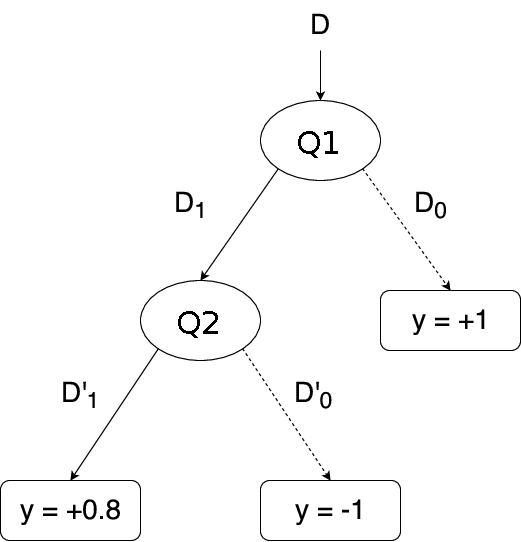
\includegraphics[width=300pt]{img/dtr_drawio.png}
\begin{textblock*}{\textwidth}(000pt,-430pt)
	\vspace*{160pt}
	入力データに対して \\
	内部ノードで質問し最適な分割を行う \\
	葉ノードで定数値を返す \\

	\vspace*{20pt}
	質問 : \\
	ある部分グラフを含むor含まない \\

	\vspace*{20pt}
	勾配ブースティングは分類木ではなく回帰木が必要 
\end{textblock*}
\begin{textblock*}{\textwidth}(925pt,-205pt)
	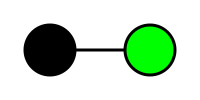
\includegraphics[width=60pt]{img/subgraph/kg.png}
\end{textblock*}
\begin{textblock*}{\textwidth}(820pt,-205pt)
	\scriptsize
	\fontsize{18pt}{0pt} \selectfont含む
\end{textblock*}
\begin{textblock*}{\textwidth}(1040pt,-205pt)
	\scriptsize
	\fontsize{18pt}{0pt} \selectfont含まない
	\end{textblock*}
\begin{textblock*}{\textwidth}(855pt,-100pt)
	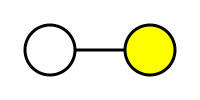
\includegraphics[width=60pt]{img/subgraph/wy.png}
\end{textblock*}
\begin{textblock*}{\textwidth}(750pt,-95pt)
	\scriptsize
	\fontsize{18pt}{0pt} \selectfont含む
\end{textblock*}
\begin{textblock*}{\textwidth}(980pt,-95pt)
	\scriptsize
	\fontsize{18pt}{0pt} \selectfont含まない
\end{textblock*}
